\input{/Users/Juste/Documents/ComplexSystems/CityNetwork/Docs/Headers/PresentationHeader.tex}



\title{Thesis Progress Meeting}


\author{J.~Raimbault$^{1,2}$}

\institute{$^{1}$G{\'e}ographie-cit{\'e}s (UMR 8504 CNRS)\\
$^{2}$LVMT (UMR-T 9403 IFSTTAR)}


\date{September 29th 2016}


%%%%%%%%%%%%%%%%%%%%%%%%%%%%%%%%
\begin{frame}
\titlepage
\end{frame}

%\begin{frame}
%\tableofcontents
%\end{frame}
%%%%%%%%%%%%%%%%%%%%%%%%%%%%%%%%



\section{Achieved Work}

% Previous
%\item SFICSSS [4w] (+ holidays [2w])\medskip
%\item Cybergeo Paper [1w]\medskip
%\item Density Paper [1w]\medskip
%\item Theoretical Paper [1w]\medskip
%\item Static Correlations (presentation at RGS conference on 31th) [1w]\medskip
%\item China project [1w]\medskip


%	(15,5exp)
%	15,2
	
%Bib/reading	1,2
%Conference	1,9
%Misc : orga, tools, discpr, cyb, monitorat, territ, NW, Energy	1,4
%Reviewing	0,3
%SFICSSS	4,7
%TransportationEquilibrium	0,3
%NwDensity	1,7
%Chine	0,2
%NetworkNecessity	1
%Holidays	2,5




\jframe{Achieved Work (by projects)}{
\begin{itemize}
\item SFICSSS [4.7w] (+ holidays [2.5w])
\item Network-Density (RGS) [1.7w] (ETA 1w)
\item Interaction Gibrat (CCS) [1w] (//th. paper, ETA 1w)
\item China [0.2w]
\item Reviewing [0.3w]
\item Transportation Eq [0.3w]
\item Biblio/reading [1.2w] ; Conference [1.9w] ; Misc [1.4w]
\end{itemize}
}




\section{Technical Developments}

\subsection{Static Correlations}


\sframe{For a Cautious Use of Big Data and Computation (RGS-AC 2016)}{
\textbf{Presentation Rationale} : \textit{Large scale computation and Big Data make no sense (are endangered) without theory and/or analytical preliminaries}

\bigskip
\bigskip

\textbf{Case Study} : \textit{Static Correlations between urban form and network measures ; insights into ergodicity and stationarity}

}





\sframe{Dataset construction}{
% brief description of nw simplification ; 

Computation of topological road network for all Europe, at 100m granularity scale (to be used consistently with population grid~\cite{eurostat})

\medskip

$\rightarrow$ Import of OSM into \texttt{pgsql}, simplification at 100m granularity, topological simplification with split/merge algorithm

\bigskip
%
%\begin{columns}
%\begin{column}{width=0.7\textwidth}
%
%\end{column}
%\begin{column}{width=0.3\textwidth}
%\textit{.} % TODO summary stats here.
%\end{column}
%\end{columns}

\begin{columns}
\begin{column}{0.7\textwidth}
    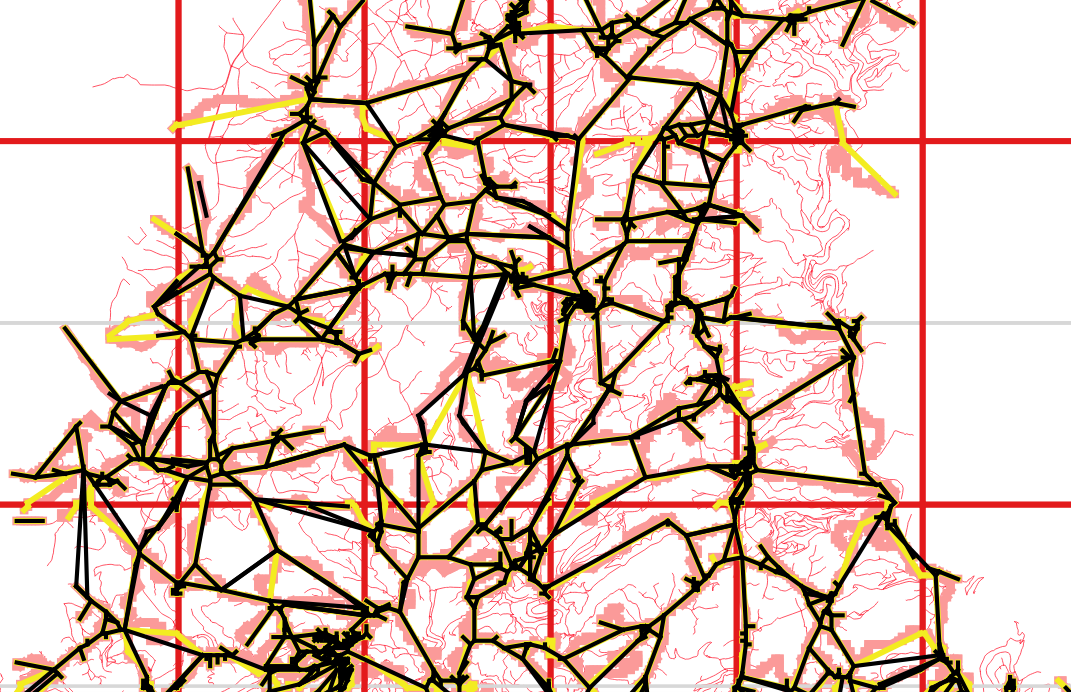
\includegraphics[width=\textwidth,height=0.5\textheight]{figures/ex_nw}
\end{column}
\begin{column}{0.3\textwidth}
   \textit{$\simeq 44\cdot 10^6$ links in initial OSM db, $\simeq 61\cdot 10^6$ in first simplified layer, $\simeq 21\cdot 10^6$ in final database}
\end{column}
\end{columns}


}



%%%%%%%%%%%%%%%%%
\sframe{Results : Computation of Indicators}{


\textit{Computation of urban form indicators~\cite{le2015forme} and network indicators on $l_0=10km$ side square}

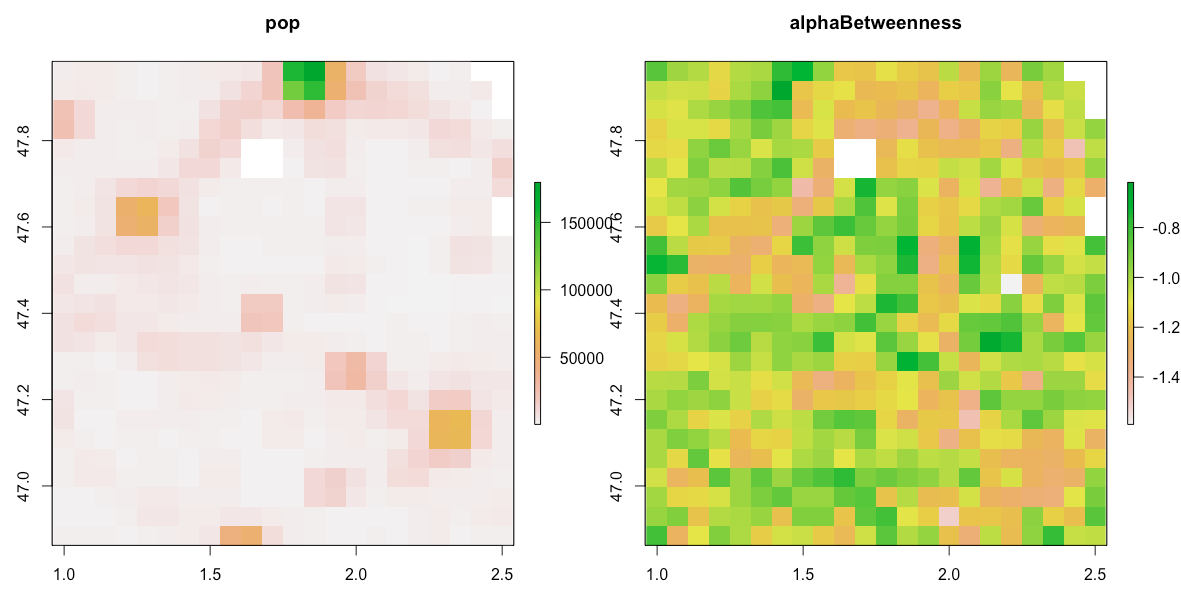
\includegraphics[width=\textwidth]{figures/pop-alphaBetweenness}

}


%%%%%%%%%%%%%%%%%
\sframe{Results : Spatial Correlations}{

\textit{Computation of spatial correlation on square areas of width $\delta\cdot l_0$ (with typically $\delta = 4, \ldots , 16$)}

\centering

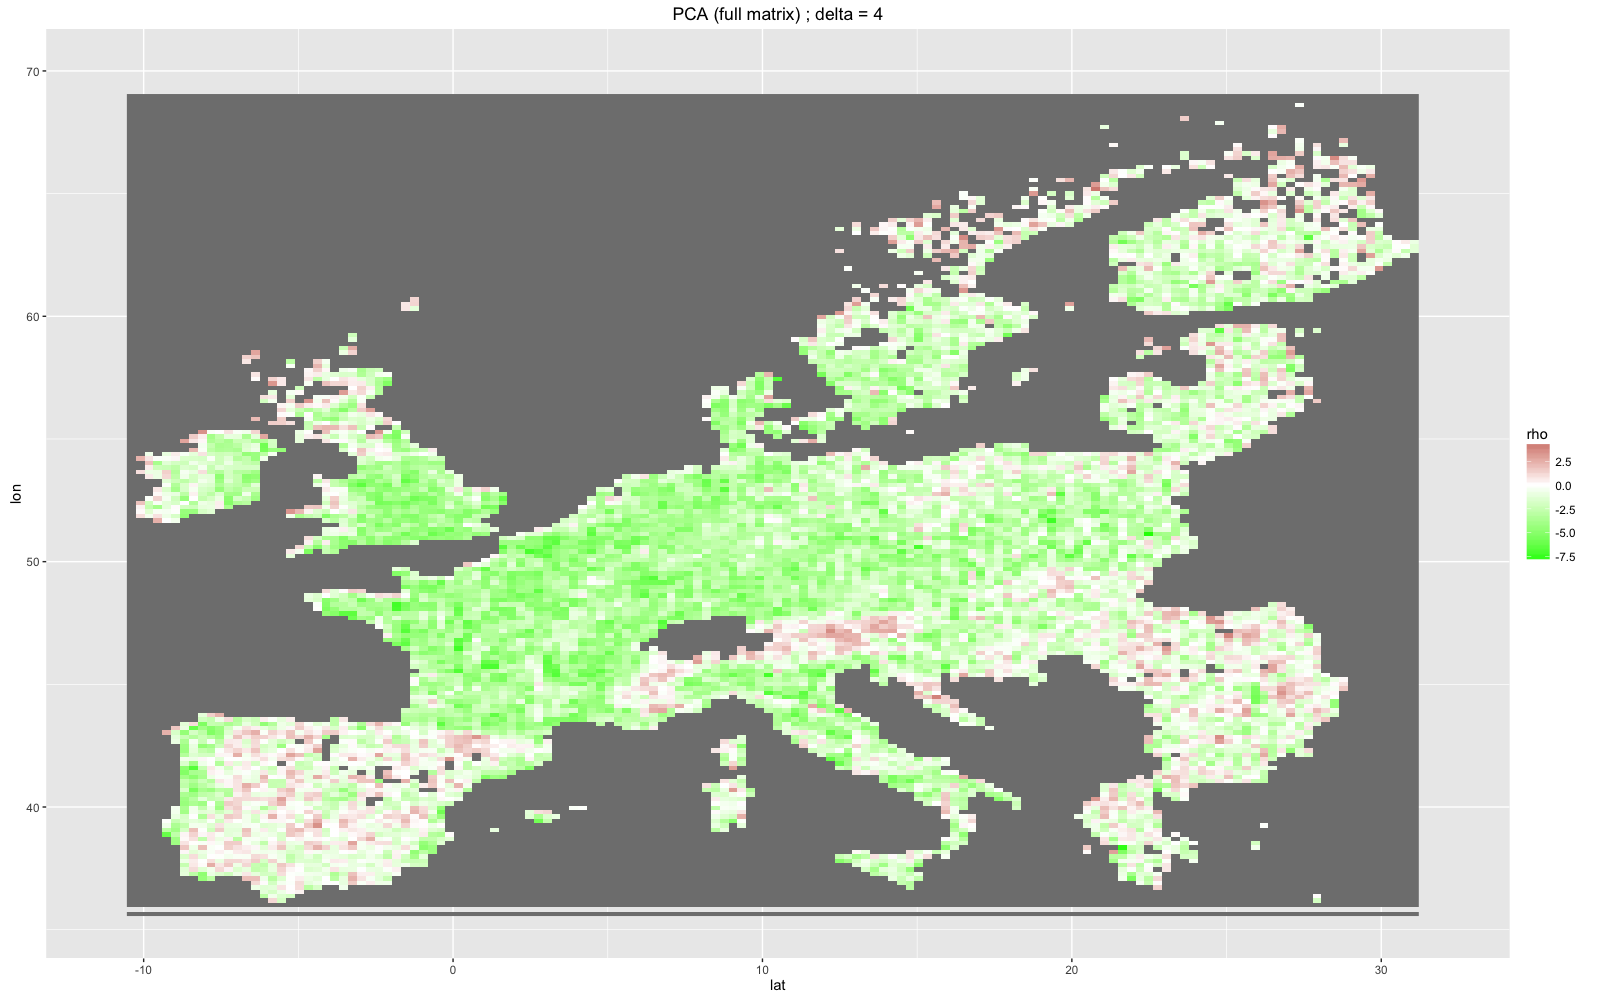
\includegraphics[width=\textwidth,height=0.7\textheight]{figures/corr_PCA_delta4}

$\rightarrow$ \textit{local spatial stationarity of processes}

}


%%%%%%%%%%%%%%%%%
%\sframe{Results : Stationarity scales}{
% maps
% 
%}



%%%%%%%%%%%%%%%%%
\sframe{Results : Multi-scale Processes}{
% plots
%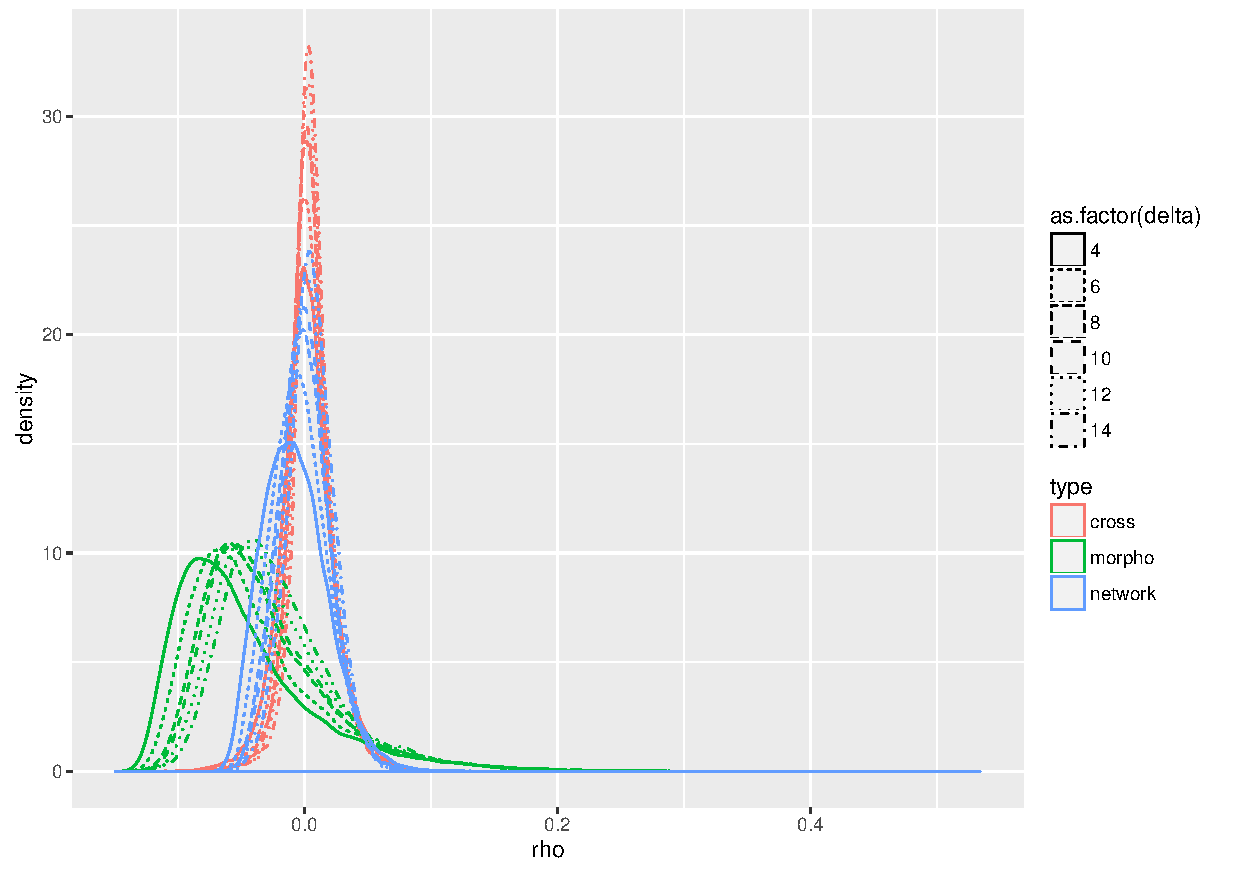
\includegraphics[width=0.33\textwidth]{figures/corrs-distrib_varyingdelta_bytype} % -> in supp material
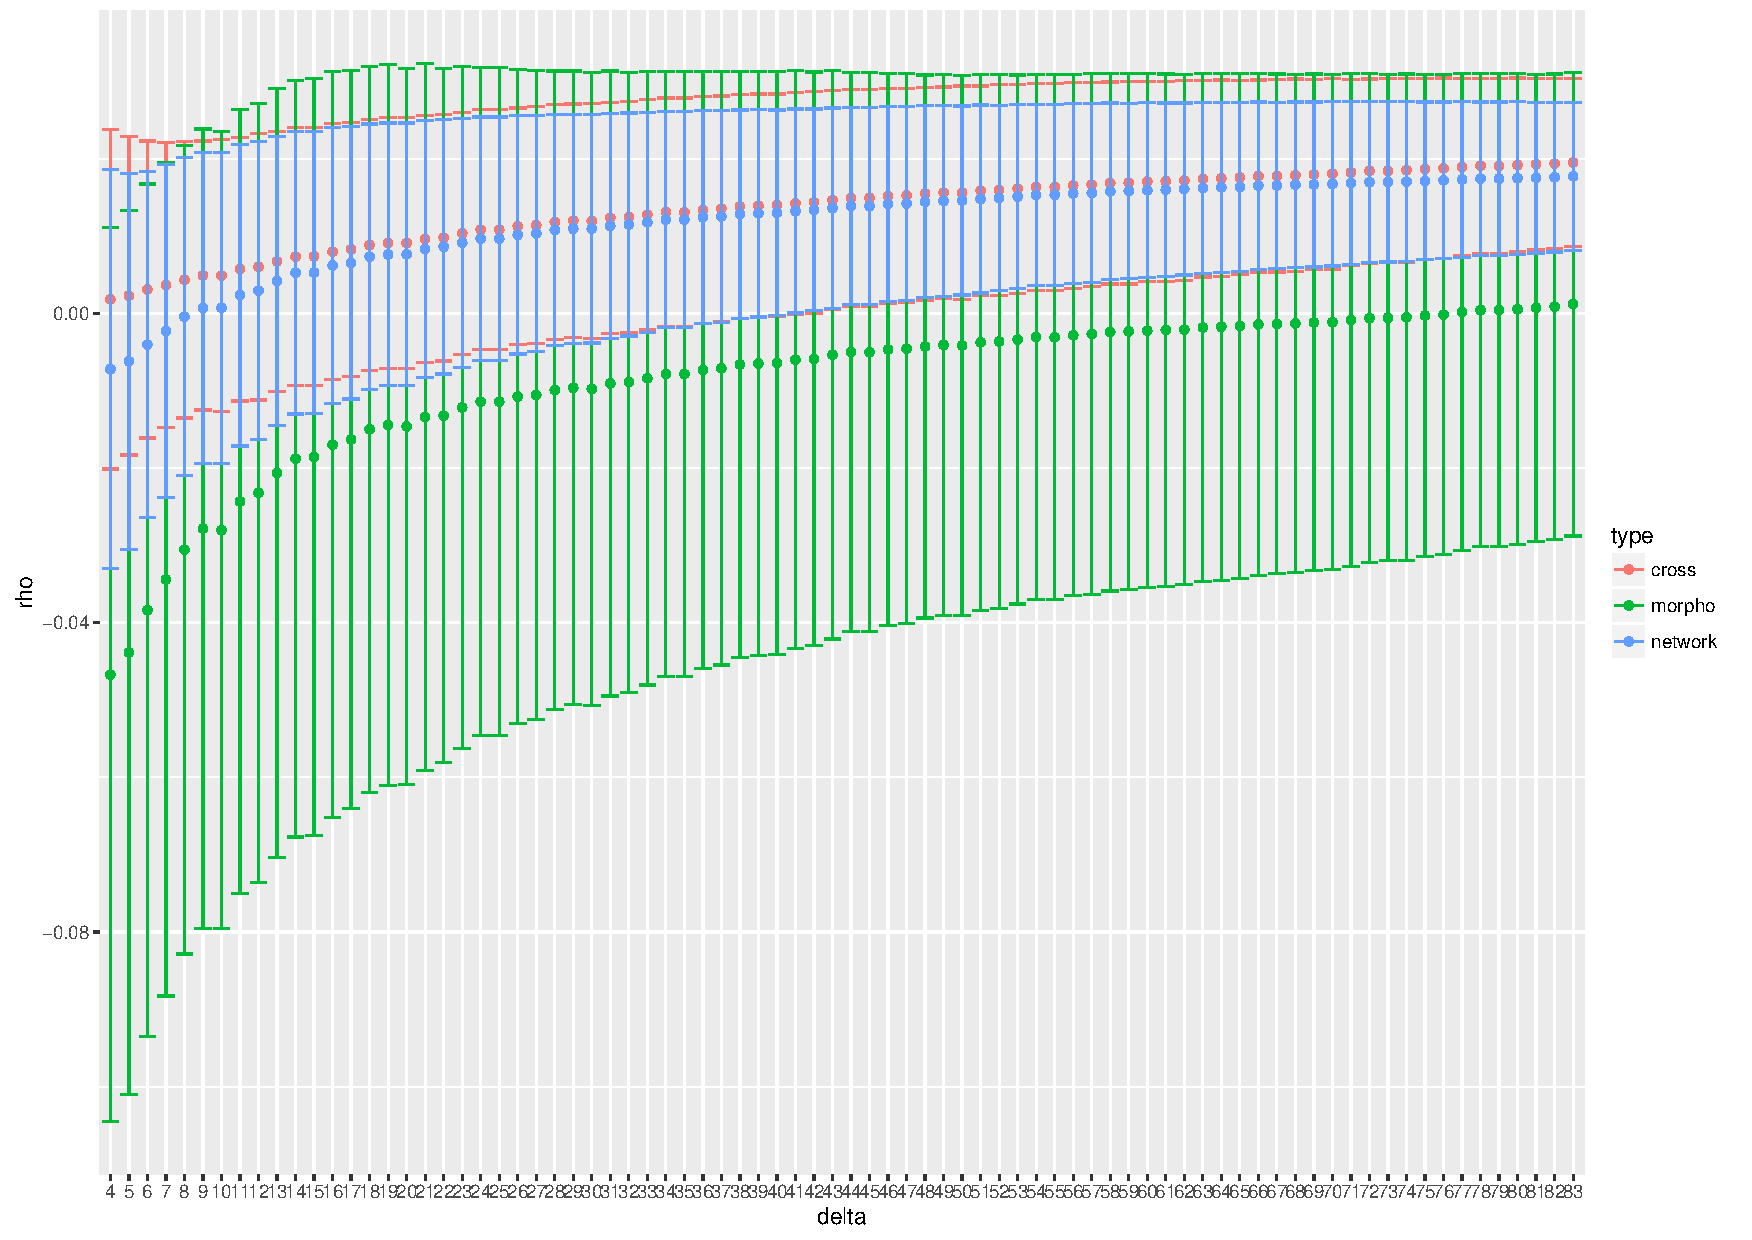
\includegraphics[width=0.5\textwidth]{figures/corrs-summary_varyingdelta_bytype_extended1}
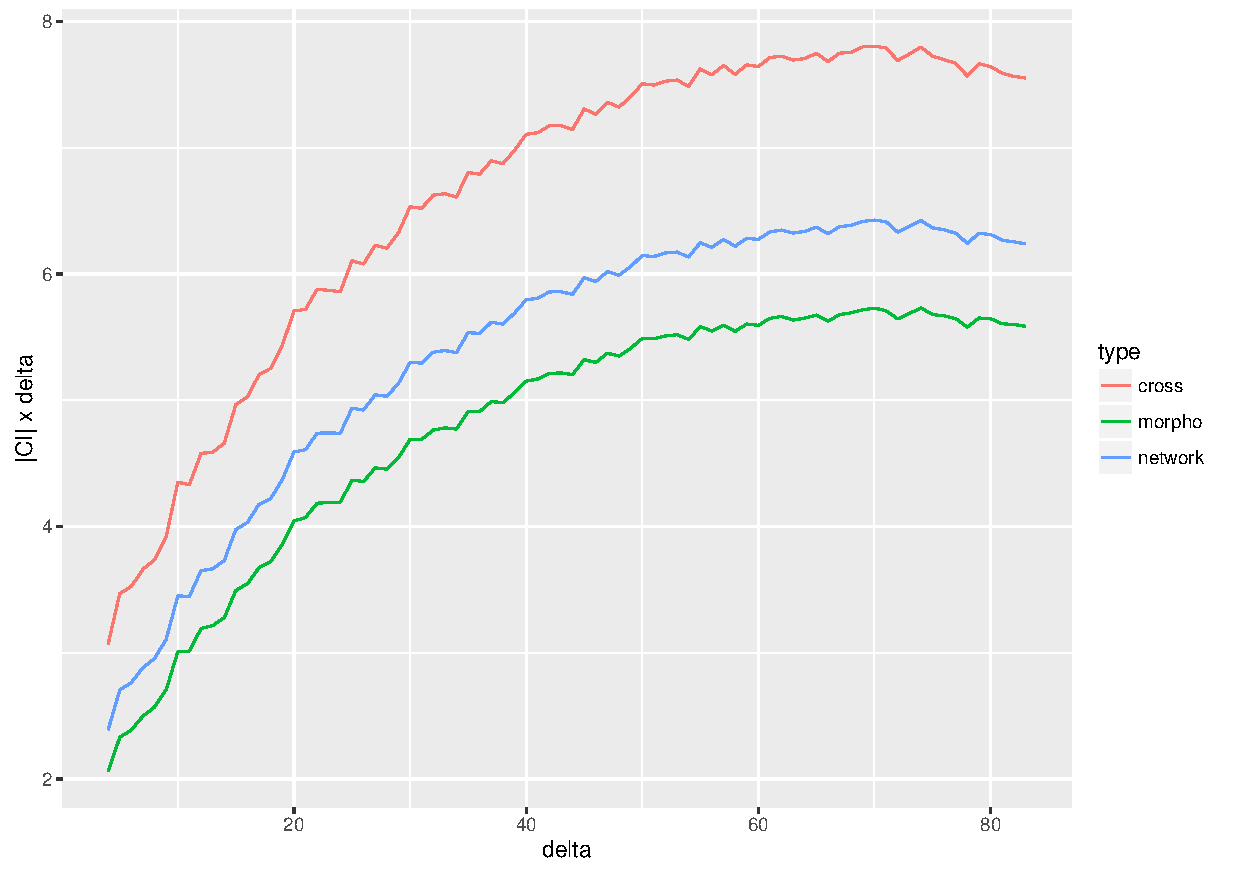
\includegraphics[width=0.5\textwidth]{figures/normalized_CI_delta}

\medskip

$\rightarrow$ Significant variation of mean correlation with $\delta$ (Left) and of normalized confidence interval (Right) given by $\left|\rho_+ - \rho_-\right|\cdot \delta$, as bounds theoretically vary as $\sqrt{N} \sim \sqrt{\delta^2}$ : implies multi-scalarity

}





\sframe{Empirical Findings (Formalization)}{

$Y_i\left[\vec{x},t\right]$ spatio-temporal stochastic process, verifies empirically :

\bigskip

\begin{enumerate}
\item Local spatial autocorrelation is present and bounded by $l_{\rho}$ (in other words the processes are continuous in space) : at any $\vec{x}$ and $t$, $\left|\rho_{\norm{\Delta \vec{x}} < l_{\rho}}\left[Y_i (\vec{x}+\Delta \vec{x},t), Y_i (\vec{x},t) \right]\right| > 0$.
\medskip
\item Processes are locally parametrized : $Y_i = Y_i\left[\alpha_i\right]$, where $\alpha_i (\vec{x})$ varies with $l_{\alpha}$, with $l_{\alpha} \gg l_{\rho}$ and weakly locally stationary in space.
\medskip
%\item Spatial correlations between processes have a sense at an intermediate scale $l$ such that $l_{\alpha}\gg l \gg l_{\rho}$.
%\item Processes covariance stationarity times scale as $\sqrt{l}$.
%\item Local ergodicity is present at scale $l$ and dynamics are locally chaotic.
\item Processes are multi-scalar : since $\rho(\delta = \infty) > \rho (\delta = 0 )$, a necessary non-linear correction on processes spatial averages in correlation computation is present.
% add computation in supplementary materials / papers. -> later
\end{enumerate}
}


\sframe{Analytical Deductions}{

1. \textbf{Regimes of temporal correlations.} Let assume local ergodicity in $\vec{x}_0$ at scale $\delta \cdot l_0$ (reasonable with urban growth and network extension in recent times). The Ergodic theorem implies that $\exists \mathcal{T}$ such that

\[<Y_i (t) >_{\norm{\vec{x}-\vec{x}_0} < \delta\cdot l_0} = <Y_i (\vec{x}_0)>_{t\in \mathcal{T}}\] 

With spatial stationarity, $<Y_i>_{\vec{x}_0}=<Y_i>_{\vec{x}_1}$, thus $\mathcal{T}$ must be constant to be invariant by translation. By contraposition and (2), processes have different dynamical characteristics.
% if translate in a given direction, looses a small part, must be compensated by the area translated by delta (overlap), thus must be constant.

\bigskip

2. \textbf{Global non-ergodicity.} Let $X_k$ a partition of space into local areas. We have $<\cdot>_x = \sum_k w_k <\cdot>_{x_k} =_{(1)} \sum_k w_k <\cdot>_{\mathcal{T}_k} $. On the other hand, global ergodicity would give $<\cdot>_t = <\cdot>_{\mathcal{T}} = \sum_k w_k <\cdot>_{\mathcal{T}}$ and $\sum_k w_k \left(<\cdot>_{\mathcal{T}} - <\cdot>_{\mathcal{T}_k}\right) = 0$. Being true on each subset implies $\mathcal{T}=\mathcal{T}_k$, what contradicts (1).


}




\subsection{Network Necessity}

\sframe{Simple Models of Growth for System of Cities (CCS 2016)}{


\textbf{Presentation Content} :

\bigskip

$\rightarrow$ \textit{Gravity/Network feedback spatial interactions models of growth : presentation and current results}

\bigskip

$\rightarrow$ \textit{Proposition of an empirical AIC methodology, application to the model}


}



\sframe{Implementation}{

\textit{On the importance of visualization in spatial models : complementary implementations in NetLogo/R/Scala}

\medskip

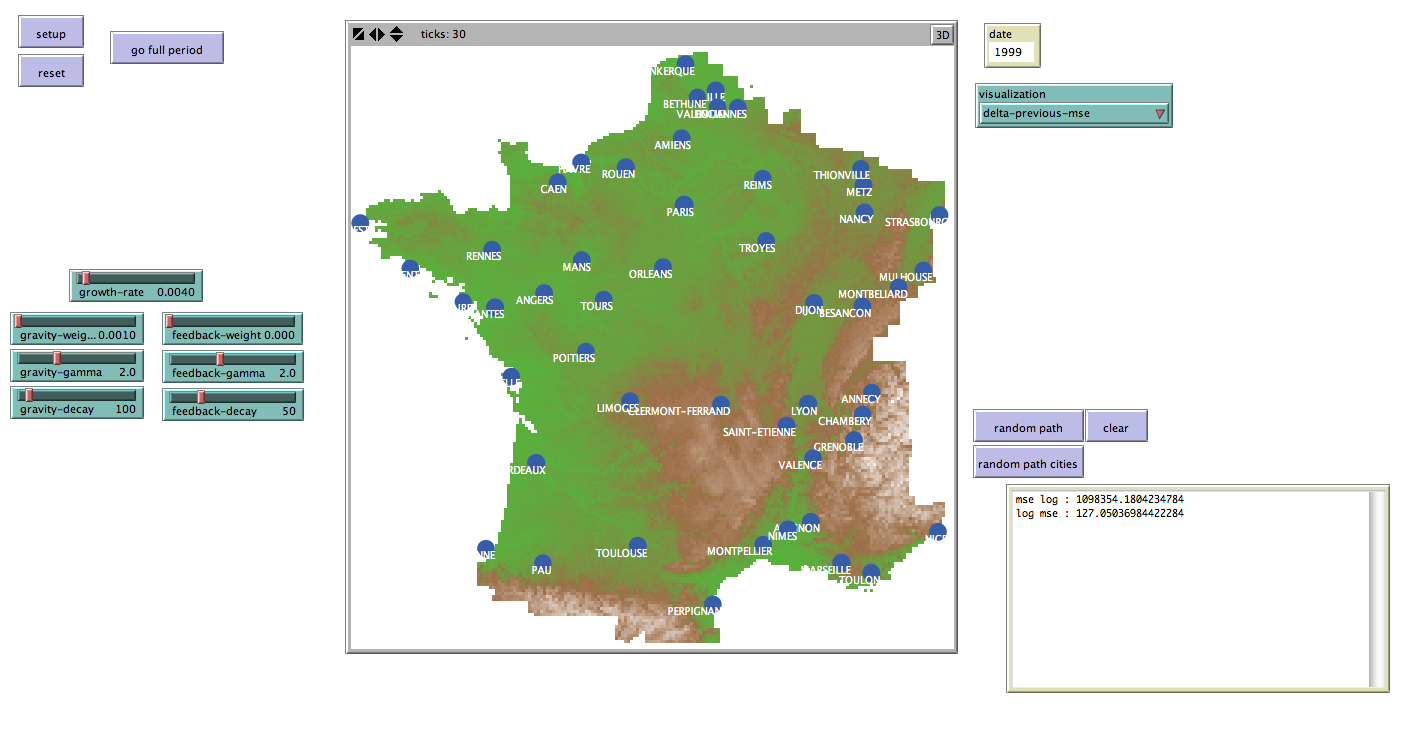
\includegraphics[width=\textwidth]{figures/example_interface}

}




\sframe{Quantifying overfitting : Empirical AIC}{

\justify

\vspace{-0.5cm}

\textit{Not clear nor well theorized how to deal with overfitting in models of simulation.} \textbf{Intuitive idea : } Approximate gain of information by approaching models of simulation by statistical models.

\medskip

Let $M_k^{\ast} = M_k\left[\alpha_k^{\ast}\right]$ computational models heuristically fitted to the same dataset. With $S_k \simeq M_k^{\ast}$, we show that $\Delta D_{KL}\left( M_k^{\ast},M_{k'}^{\ast}\right) \simeq \Delta D_{KL}\left( S_k,S_{k'}\right)$ if fits of $S_k$ are negligible compared to fit difference between computational models and models have same parameter number.

\bigskip

\textbf{Application} $M_1$ : gravity only model with $(r_0=0.0133,w_G=1.28e-4,\gamma_G=3.82,d_G=4e12)$ ; $M_2$ : full model with $(r_0=0.0128,w_G=1.30e-4,\gamma_G=3.80,d_G=8.4e14,w_N=0.603,\gamma_N=1.148,d_N=7.474)$

Fitting of independent polynomial models ($\tilde{P}_i(t) = Q\left[\tilde{P}_i(t-1)\right]$) with 4 and 7 parameters) gives $\Delta D_{KL} \simeq 19.7$ $\rightarrow$ fit improvement without overfitting


}









\section{China Project}

\sframe{Extension/Application of Lutecia model}{

$\rightarrow$  Empirical description of governance structure for transportation within the MCR, associated issues.

\bigskip

$\rightarrow$ Application of the model to the real case (after refined exploration, sensitivity analysis and internal validation).

\bigskip

$\rightarrow$  Focus on specific questions involving the medium-sized city of Zhuhai : position and influence within MCR processes ; specific governance configuration (the city is a Special Economic Zone e.g.).



}


\sframe{Towards a SimpopSino model}{

$\rightarrow$ Extension of Gibrat-Interaction model, taking into account at least one economic dimension

\bigskip

$\rightarrow$ Meeting with Denise : ok for Elfie dataset ; importance of link meso-macro in transportation

\bigskip

$\rightarrow$ Rapidly growing network in China

\cite{kenworthy2002transport,lyu2016developing} : 

construction of a dynamical database ; test static/dynamic/co-evolution network extensions for SimpopSino


}




\section{Next Steps}


%%%%%%%%%%%%%%%%%%%%%%%%%%%%%%%%
\jframe{Next steps (until December 15th 2016)}{
\begin{itemize}
\item Lutecia : model [3w] ; fieldwork [2w]\medskip
\item SimpopSino : theoretical/modeling [3w] \medskip
\item Thesis/papers writing [2w]
\end{itemize}
}



\jframe{Thesis Organisation (remainder)}{
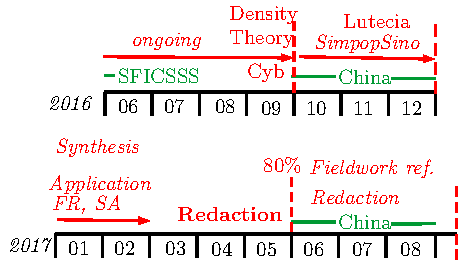
\includegraphics[width=\textwidth]{figures/edt}
}







%%%%%%%%%%%%%%%%%%%%%%%%%%%%%%%%
\begin{frame}[allowframebreaks]
\frametitle{References}
\bibliographystyle{apalike}
\bibliography{/Users/Juste/Documents/ComplexSystems/CityNetwork/Biblio/Bibtex/CityNetwork}
\end{frame}
%%%%%%%%%%%%%%%%%%%%%%%%%%%%%%%%


\end{document}






